% ---
% Capa
% ---
\imprimircapa
% ---

% ---
% Folha de rosto
% (o * indica que haverá a ficha bibliográfica)
% ---
\imprimirfolhaderosto*
% ---

% ---
% Inserir a ficha bibliografica
% ---
% http://ficha.bu.ufsc.br/
\begin{fichacatalografica}
	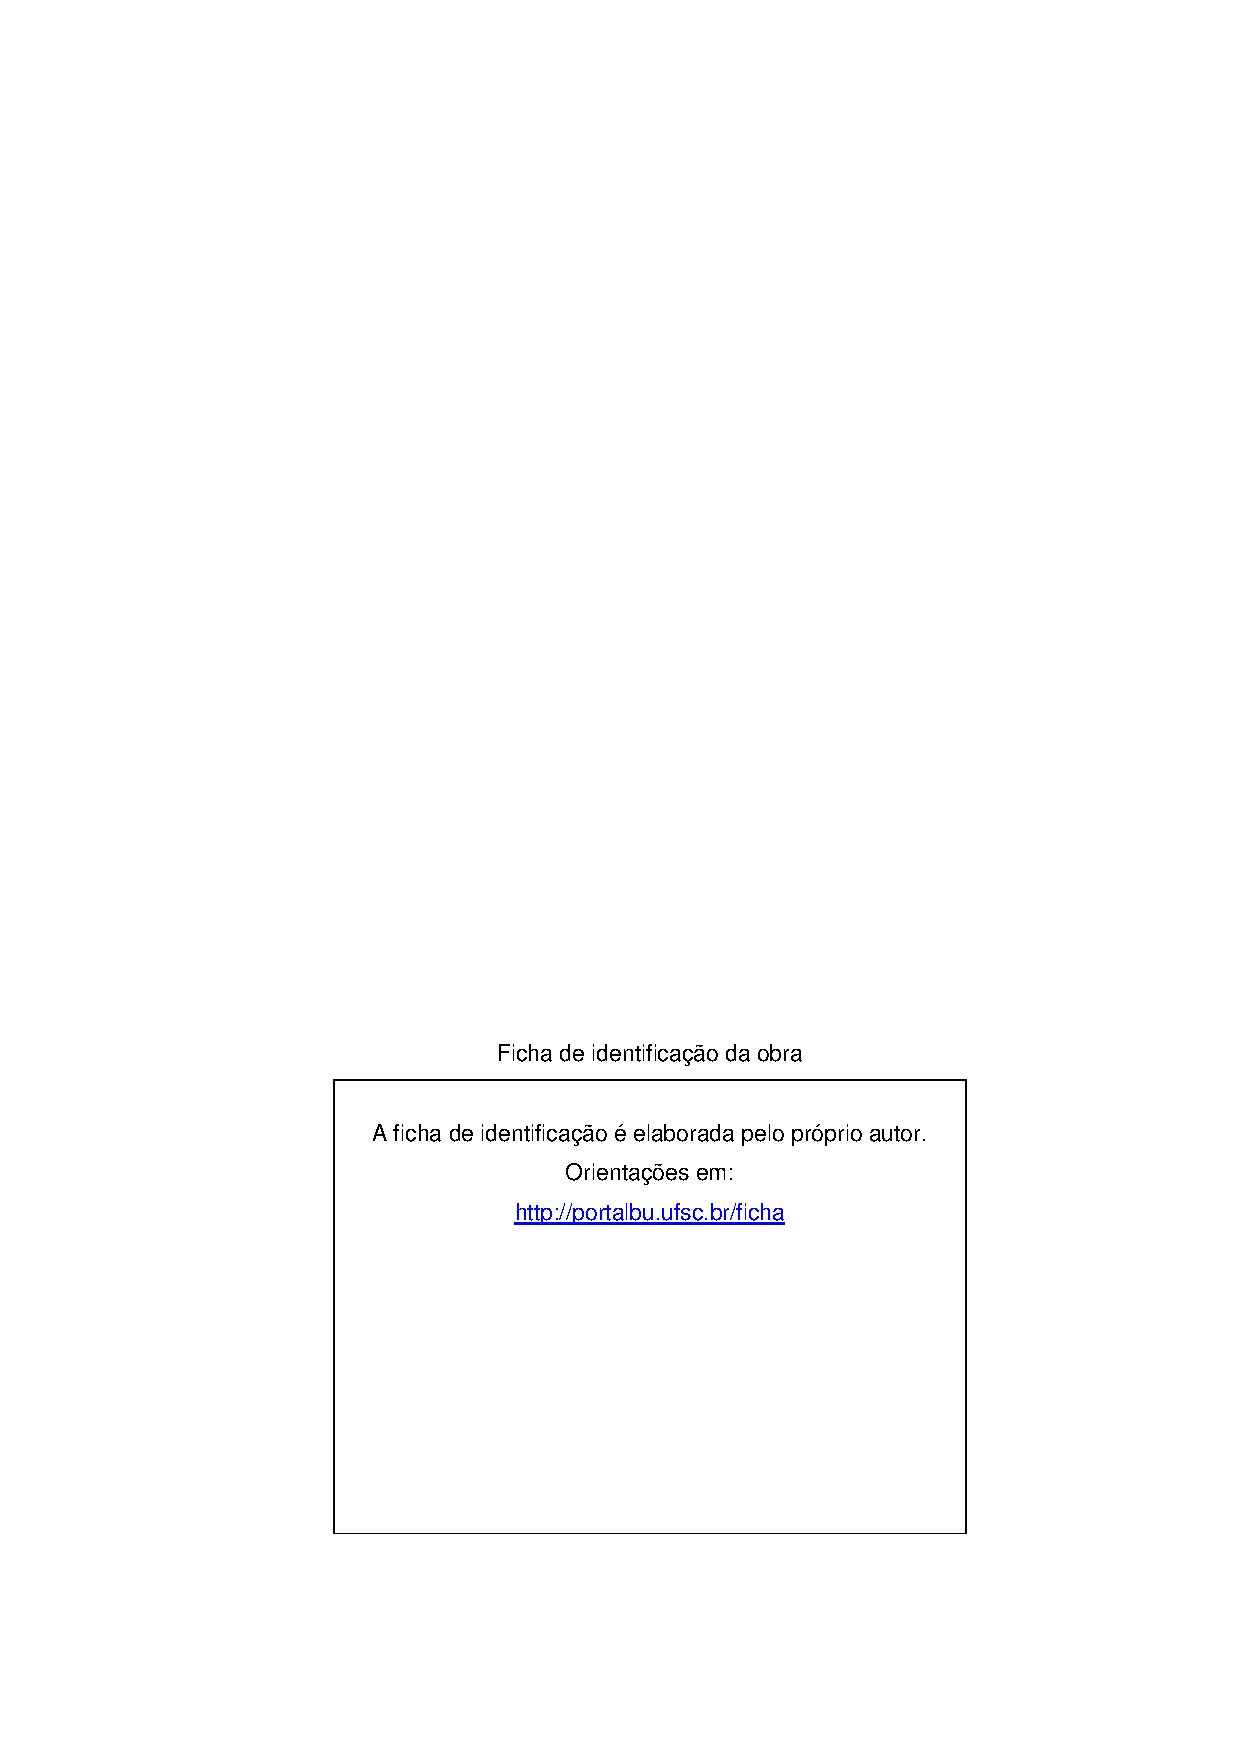
\includepdf{beforetext/Ficha_Catalografica.pdf}
\end{fichacatalografica}
% ---

% ---
% Inserir folha de aprovação
% ---
\begin{folhadeaprovacao}
	\OnehalfSpacing
	\centering
	\imprimirautor\\%
	\vspace*{10pt}		
	\textbf{\textsf{\imprimirtitulo}}%
	\ifnotempty{\imprimirsubtitulo}{:~\imprimirsubtitulo}\\%
	%		\vspace*{31.5pt}%3\baselineskip
	\vspace*{\baselineskip}
	%\begin{minipage}{\textwidth}
	% O presente trabalho em nível de \imprimirnivel~foi avaliado e aprovado por banca examinadora composta pelos seguintes membros
    O presente trabalho em nível de \imprimirnivel~foi avaliado e aprovado por banca examinadora composta pelos seguintes membros:\\
	%\end{minipage}%
	\vspace*{\baselineskip}
	Prof. Fabiano Hartmann Peixoto, Dr.\\
	Universidade de Brasilia\\
	\vspace*{\baselineskip}
	Prof. Eric Aislan Antonelo, Dr.\\
	Universidade Federal de Santa Catarina\\
	\vspace*{\baselineskip}

	Prof. Marcelo Ricardo Stemmer, Dr.\\
	Universidade Federal de Santa Catarina\\
	\vspace*{1\baselineskip}
	\begin{minipage}{\textwidth}
		Certificamos que esta é a \textbf{versão original e final} do trabalho de conclusão que foi julgado adequado para obtenção do título de \imprimirformacao.\\
% 		Certificamos que esta é a \textbf{versão original e final} do trabalho de conclusão que foi julgado adequado para obtenção do título de \imprimirformacao.\\
	\end{minipage}
	
	\vspace*{\fill}
	
	\assinatura{\OnehalfSpacing Prof. Werner Kraus Junior, Dr.\\Coordenador do curso de Pós-Graduação em Engenharia de Automação e Sistemas}
	
	\vspace*{\fill}
	
	\assinatura{\OnehalfSpacing\imprimirorientador \\ Orientador}
	


	\vspace*{\fill}
	
	\imprimirlocal, \imprimirano.
\end{folhadeaprovacao}
% ---

% ---
% Dedicatória
% ---
\begin{dedicatoria}
	\vspace*{\fill}
	\noindent
	\begin{adjustwidth*}{}{0cm} 
		\raggedleft To God, my family and friends. 
	\end{adjustwidth*}
\end{dedicatoria}
% ---

% ---
% Agradecimentos
% ---
\begin{agradecimentos}
I thank God for everything, but mainly for allowing me to work on this research amidst so many tribulations and for having completed this step.

I also thank my family, especially my parents and my brother, Gilmar, Rosane, and Gabriel, for all their love, support, and patience during the Master's period.

I thank my advisor, Professor Jomi Fred Hübner, PhD., for all his commitment, dedication, and willingness to guide me during the Master's period and, mainly, for showing me the way to grow as a researcher.

I would like to thank my co-supervisor, Professor Aires José Rover, PhD., also for his commitment, dedication, and willingness during the Master's period, for showing the research from another angle, and also for allowing the use of the EGOV's high-performance computer, without which this work would not be possible. 

I need to thank Isabela, Msc., a doctoral student in law, my right-hand man during this research, whether in times of bad results from experiments, in the data collection, in the paper writing, or in times of joy when receiving their acceptance. 

I must thank my colleagues in the EGOV group, for the moments of relaxation and the shared experiences, knowledge, and techniques for scientific research. 

I thank the professors, colleagues, and servants of the Automation and Systems Department at UFSC, for all the shared knowledge and assistance provided. 

I thank the Judge Vânia Petermann, from the Special Civel Court at the Federal University of Santa Catarina for allowing the research to be conducted by providing access to the court's data.

I thank everyone who in some way provided assistance during the research period but were not explicitly named. 

Finally, I would like to thank CAPES and Petrobras for allowing this work to be carried out through the granting of a master's scholarship. 


 
\end{agradecimentos}
% ---

% ---
% Epígrafe
% ---
\begin{epigrafe}
	\vspace*{\fill}
	\begin{flushright}
		\textit{``Fortitude is the disposition of soul\\
		which enables us to despise all inconveniences \\
		and the loss of things not in our power''\\
		(St. Augustine, 354-430)}
	\end{flushright}
\end{epigrafe}
% ---



\setlength{\absparsep}{18pt} % ajusta o espaçamento dos parágrafos do resumo
\begin{resumo}[Resumo]
\SingleSpacing
De acordo com o último relatório Justiça em Números, publicado anualmente pelo Conselho Nacional de Justiça, 77,1 milhões de processos aguardavam solução no Judiciário brasileiro, sendo 5,2 milhões nos Juizados Especiais Civeis (JECs). Esses números vêm crescendo ano a ano, o que indica a necessidade de criação de mecanismos para auxiliar o Judiciário brasileiro a ser mais célere e eficaz. Assim, este trabalho visa contribuir nesse cenário aplicando as técnicas de Aprendizado de Máquina (ML) e Mineração de Textos (TM) para a previsão dos resultados dos julgamentos do JEC localizado na Universidade Federal de Santa Catarina, relacionados  a falhas nos serviços de transporte aéreo. Para isso, dividimos o problema em três partes: representação, classificação e regressão. Na primeira parte,  avaliamos a possível influência do tamanho e a especificidade dos \textit{corpora} usados para treinar \textit{word embeddings} sobre o desempenho da classificação de textos. Desse modo, \textit{word embeddings} foram treinados com base em julgamentos em português. Como resultado, descobrimos que tamanho e especificidade importam, porém o tamanho influencia os resultados até certo ponto. Na segunda parte, avaliamos se as técnicas de Aprendizado Profundo (DL) apresentam melhor desempenho do que as técnicas de ML Clássico na predição dos resultados dos julgamentos do JEC. Assim, treinamos várias técnicas de DL e ML Clássico usando dois tipos de conjunto de dados, um contendo o texto completo dos julgamentos e outro com a parte do dispositivo removida. No primeiro caso, as técnicas de DL apresentam melhor desempenho, o que significa que podem assimilar melhor as partes dos textos que explicitamente indicam o resultado. Neste último, as técnicas clássicas tiveram melhor desempenho, indicando que sem a parte do resultado estar explícita, essas técnicas podem melhor aprender como classificar a partir das demais partes do processo. Na terceira parte, nos concentramos em prever o valor da indenização por danos morais, usando técnicas de regressão. Com base em vários pipelines e na avaliação de um especialista em direito, percebemos que a qualidade de predição alcançada em tal tarefa é aceitável e pode ser útil no domínio jurídico. Assim, concluímos que foi possível prever com precisão os resultados dos julgamentos do JEC e o valor da indenização por danos morais utilizando os \textit{pipelines} propostos. 

\textbf{\textsf{Palavras-chave}}: Aprendizado de Máquina. Classificação de Texto. Representação de Texto. Regressão de Texto. Juizado Especial Cível. Decisões Judiciais.
\end{resumo}




\setlength{\absparsep}{18pt} % ajusta o espaçamento dos parágrafos do resumo
\begin{resumo}[Resumo Expandido]
	\SingleSpacing
	
\textbf{\textsf{INTRODUÇÃO}}


De acordo com o último relatório \textit{Justiça em Números}, publicado anualmente pelo Conselho Nacional de Justiça (CNJ), ao final de 2019 havia cerca de 77,1 milhões de processos em andamento aguardando solução no Judiciário brasileiro. No total, em 2019, foram 30,2 milhões de ações ajuizadas em todo o Judiciário, um aumento de 6,8\% em relação a 2018. Dessas ações, cerca de 5,2 milhões foram ajuizadas nos Juizados Especiais Cíveis (JEC) \cite{CNJ2020}.  Para fazer face aos desafios enfrentados nos sistemas judiciários no Brasil e no mundo \cite{Sadiku2020}, é cada vez maior o interesse da literatura em aplicar técnicas baseadas em aprendizado de máquina e mineração de textos na área jurídica. Os artigos publicados buscam solucionar diversos problemas jurídicos, como extração de informações de contratos \cite{Hassan2020} e previsão de decisões em tribunais inferiores e superiores \cite{Sulea2017, Virtucio2018}. O aprendizado de máquina se concentra na construção de sistemas de computador que aprendem por meio da experiência \cite{Mitchell1997}, enquanto a mineração de textos está relacionada à ideia de descobrir e analisar padrões, como tendências e outliers, a partir de dados textuais. Mineração de textos também se concentra em ajudar os usuários a analisar e digerir informações para uma melhor tomada de decisão \cite{Aggarwal2013}. 
Considerando o alto nível de judicialização no Brasil, menos casos são decididos por meio de acordos entre as partes e, por isso, essas têm de esperar pelo julgamento de um juiz, o que pode levar de dias a anos \cite{Cury2019, Mancuso2020}.
Se as partes possuíssem mais informações sobre os possíveis resultados de seus processos, baseadas em julgamentos anteriores do juíz, elas poderiam encerram o caso ainda na conciliação. Além disso, nos JECs, as decisões ainda são manuais, sem nenhum tipo de automação. O mesmo vale para decisões envolvendo danos morais, onde não há critérios claros para definição dos valores, dependendo muito da interpretação do juiz a cerca do caso.
    Portanto, este trabalho pretende contribuir para o estado da arte em aprendizado de máquina e em mineração de textos através da investigação de soluções para predição dos possíveis resultados de processos. Tais processos são provenientes do JEC localizado na Universidade Federal de Santa Catarina e envolvem falhas em serviços de transporte aéreo. No entanto, para tal predição ocorra, três desafios são colocados: a representação numérica de textos jurídicos, necessária para a aplicação destes em algoritmos de aprendizado de máquina, levando em conta sua complexidade e vocabulário próprios. Porém, não há trabalhos explorando a representação de textos jurídicos em português a partir de técnicas como o \textit{word embeddings}. O segundo desafio se refere à predição do resultado do processo, através da tarefa de classificação, onde pretende-se treinar um modelo capaz de mapear um conjunto de dados para um conjunto de finito de rótulos. O terceiro se refere ao uso de regressão para predição do valor do dano moral a partir do texto do processo. No entanto, a partir de uma revisão da literatura, pode se afirmar que regressão ainda não foram aplicadas a textos jurídicos.

\textbf{\textsf{OBJETIVOS}}

Com base na problemática de predição do resultado dos processos do JEC na UFSC, o objetivo do trabalho é avaliar se é possível prever o julgamento final do caso a partir do seu texto e prever o valor de indenização por danos morais usando técnicas de aprendizado de máquina e mineração de textos. E, para levantar possíveis soluções para os três desafios, três objetivos específicos precisam ser executados. O primeiro deles se refere à representação, onde busca avaliar se o tamanho e a especifidade dos \textit{corpora} usados para treinar modelos de \textit{word embeddings} impacta na performance na tarefa classificação de textos. O segundo a partir dos resultados do primeiro busca avaliar se técnicas de aprendizado profundo superam técnicas clássicas de aprendizado de máquina na predição do resultado dos julgamentos do JEC. E, por fim, o terceiro objetivo se refere à regressão, onde busca-se avaliar se a predição de indenização por danos morais pode ser precisa e útil no ambiente jurídico a partir do uso de regressão em textos.


\textbf{\textsf{MÉTODO DE PESQUISA}}


Para cumprir os objetivos, o pesquisador seguiu um conjunto de passos aos quais são similares para cada objetivo específico, com pequenas distinções.
Anteriormente à definição do problema, pergunta de pesquisa e objetivo de cada uma das três partes, construiu-se três Revisões Sistemáticas da Literatura (RSL) para identificar o estado arte em relação a aplicação de aprendizado de máquina e mineração de textos no direito e o uso de técnicas de representação e regressão no direito.
O passo seguinte consistiu na coleta das bases textuais necessárias para cumprir os objetivos. Tais conjuntos de dados incluiram bases textuais de acórdãos de tribunais superiores bem como julgamento do JEC. Por fim, com o ajuda da especialista em direito, foram extraídos atributos a cerca dos processos.
O terceito passo se refere à construção de experimentos de aprendizado de máquina e mineração de texto para cada objetivo.
O quarto passos se refere à avaliação dos resultados obtidos e discussão.


\textbf{\textsf{RESULTADOS E DISCUSSÃO}}

Os três conjuntos de experimentos realizados buscaram atingir os três objetivos propostos. Em relação à representação, discutiu-se o impacto do tamanho e especificade dos \textit{corpora} usado para treinar \textit{word embeddings} na performance na classificação de textos. Percebeu-se que tanto tamanho e especificidade importam. No entanto, em termos de tamanho, percebeu-se que este impacta até um certo ponto de tal forma que adicionar mais texto não traz impactos significativos. Em relação à classificação, buscou-se comparar como técnicas de aprendizado profundo e clássicas se desempenhavam na predição dos resultados dos processos do JEC e se a primeira traria resultados superiores em relação à segunda. Percebeu-se que técnicas de aprendizado clássico se saem melhor quando o texto do julgamento não apresenta a seção de dispositivo, enquanto técnicas de aprendizado profundo performaram melhor quanto tal seção estava presente. Portanto, a aplicação real da predição no JEC usaria técnicas clássicas. Em relação aos experimentos com  regressão, percebeu-se que, a partir de aprimoramentos na pipeline para predição do valor de indenização, pode-se obter resultados com qualidade aceitável para o ambiente jurídico, uma vez que o erro médio absoluto atingido foi de menos de mil reais. Portanto, com base nos resultados alcançados, é pode se afirmar que a predição do resultado e da indenização por danos morais em julgamentos do JEC é possível a partir de técnicas aprendizado de máquina e de mineração de textos.

\textbf{\textsf{CONSIDERAÇÕES FINAIS}}

A cada ano, o número de processos judiciais aguardando decisão final tende a aumentar. Portanto, é fundamental encontrar soluções para agilizar o Judiciário brasileiro em suas diversas instâncias, desde os Juizados Especiais Cíveis até o Supremo Tribunal Federal.
Neste trabalho, é proposta a aplicação das técnicas de mineração de textos e aprendizado de máquina em julgamentos do Juizado Especial Civel da UFSC para prever os possíveis resultados bem como o valor da indenização por danos morais. Assim, esta pesquisa visa contribuir para o aumento de acordos em audiências de conciliação nos juizados especiais. 
O objetivo e a pergunta de pesquisa se refereriram à possibilidade de se prever o resultado dos julgamentos do JEC a partir do seu conteúdo, bem como  o valor de indenização por danos morais. Para tanto, três desafios foram colocados para que se atingisse o objetivo geral, sendo eles a representação de textos jurídicos, a predição do resultado do julgamento, a partir de classificação e a predição da indenização por dano moral, a partir de regressão.
Em relação à representação discutiu-se o impacto do tamanho e especificidade dos \textit{corpora} para treinamento de \textit{word embeddings} na performance classificação e percebeu-se que havia influência de ambos, no entanto o tamanho apenas até certo ponto. Em relação à classificação,  percebeu-se que a predição de julgamentos do JEC foi melhor executada por técnicas clássicas de aprendizado de máquina em relação ao aprendizado profundo. Já em relação à predição de indenização por danos morais atingiu resultados aceitáveis dentro do ambiente jurídico a partir de aprimoramentos como N-Grams e atributos extraídos pela especialista em direito. Em relação ao objetivo geral, pode-se concluir que é possível prever o resultado do julgamento a partir do texto, uma vez que a melhor acurácia foi de 82,2\%. Também é possível atingir resultados acuráveis na predição de indenização por danos morais a partir de regressão com o uso dos aprimoramento sugeridos.
Como trabalhos futuros, almeja-se verificar como técnicas de representação mais recentes influenciam nos resultados de classificação e regressão. Além disso, pretende-se verificar se é possível prever o resultado e o valor de indenização a partir do uso de textos de petições iniciais. Por fim, pretende-se aprimorar os modelos criados para que as predições sejam \textit{explicáveis} e incluir mecanismos para mitigar de eventuais vieses e preconceitos que possam estar presentes na base de dados.


\textbf{\textsf{Palavras-chave}}: Aprendizado de Máquina. Classificação de Texto. Representação de Texto. Regressão de Texto. Juizado Especial Cível. Decisões Judiciais.
\end{resumo}

% resumo em inglês
\begin{resumo}[Abstract]
	\SingleSpacing
	\begin{otherlanguage*}{english}
	
According to the last report \textit{Justiça em Números}, annually published by the National Council of Justice, 77.1 million processes were waiting for a solution in the Brazilian judiciary, of which 5.2 million in the Special Civel Courts (JECs). Those numbers have been increasing year after year, indicating the need of creating mechanisms toto help the Brazilian Judiciary to be faster and more effective. Thus, this work aims to contribute in this scenario by applying Machine Learning (ML) and Text Mining (TM) techniques to the prediction of the results of the legal judgments from the JEC located at the Federal University of Santa Catarina, which relate to failures in air transport services. To do so, we divided the problem into three parts: representation, classification, and regression. In the first part, we evaluate whether the size and specificity of the corpora used to train word embeddings, impact the performance of text classification. We, thus, trained embeddings based on judgments in Portuguese. As a result, we discovered that size and specificity matter, however size influences the results until a certain point. In the second part, we evaluate whether Deep Learning (DL) techniques perform better than Classical ML techniques in the classification of the judgments' results from JEC. Thus, we trained several DL and Classical ML techniques using two types of the dataset, one containing the full text of the judgments and another with the result part removed. In the former, the DL techniques performed better, implying that they can better assimilate the parts  of the texts that explicitly indicate the result. In the latter, classical techniques performed better, indicating that without the explicit result part, those techniques can better learn from the other parts. In the third part, we focus on predicting the compensation value for immaterial damage, using regression techniques. Based on several pipelines and on a legal expert's evaluation, we noticed that the prediction quality achieved in such a task is acceptable and it can be helpful in the legal domain. Thus, we concluded that it was possible to accurately predict the results of the judgments from JEC and the compensation value for immaterial damage using the proposed pipelines.


\textbf{\textsf{Keywords}}: Machine Learning. Text Classification. Text Representation. Text Regression. Special Civel Court. Legal Judgments.
	\end{otherlanguage*}
\end{resumo}

{%hidelinks
	\hypersetup{hidelinks}
	% ---
	% inserir lista de ilustrações
	% ---
	\pdfbookmark[0]{\listfigurename}{lof}
	\listoffigures*
	\cleardoublepage
	% ---
	
	% ---
	% inserir lista de quadros
	% ---
	%\pdfbookmark[0]{\listofquadrosname}{loq}
	%\listofquadros*
	%\cleardoublepage
	% ---
	
	% ---
	% inserir lista de tabelas
	% ---
	\pdfbookmark[0]{\listtablename}{lot}
	\listoftables*
	\cleardoublepage
	% ---
	
	% ---
	% inserir lista de abreviaturas e siglas (devem ser declarados no preambulo)
	% ---
	\imprimirlistadesiglas
	% ---
	
	% ---
	% inserir lista de símbolos (devem ser declarados no preambulo)
	% ---
	% \imprimirlistadesimbolos
	% ---
	
	% ---
	% inserir o sumario
	% ---
	\pdfbookmark[0]{\contentsname}{toc}
	
	\tableofcontents*
	\cleardoublepage
	
}%hidelinks
% ---